\documentclass[12pt,a4paper]{article}
\usepackage{ucs}
\usepackage[utf8x]{inputenc}
\usepackage{amsmath}
\usepackage{graphicx}
\usepackage{wrapfig}

\title{Osnove Mehatronike 3. lab}
\newcommand{\brvjezbe}{3}
\newcommand{\ime}{Niko Višnjić}
\newcommand{\jmbag}{0036449299}
\newcommand{\grupa}{unknown}
\newcommand{\predmet}{Osnove mehatronike} 
\newcommand{\fakultet}{Fakultet elektrotehnike i računarstva Zagreb} 
\newcommand{\zavod}{Zavod za elektrostrojarstvo i automatizaciju } 
\newcommand{\imevjezbe}{Vježba 3: Regulacija brzine vrtnje rotacijskog
elektromehaničkog sustava SRV02 \newline
-implementacija i provjera sinteze regulatora-}
\usepackage[hmargin={3.5cm,2.5cm},height=25.5cm]{geometry}
\input{"zaglavlje.tex"}
\setcounter{secnumdepth}{4}

\DeclareMathSizes{12}{12}{10}{12}

\begin{document}
\section{Uvod}
U okviru ove vježbe obavljamo pokus koji obuhvaća proces implementacije
(rad u realnom vremenu) regulatora brzine vrtnje projektiranog i simuliranog sustava tokom druge laboratorijske vježbe. 

Koristi se Simulink/WinCon okruženje kao programski razvojni alat. Postupak provjere obuhvaća usporedbu dobivenih rezultata testiranja s regulacijskim zahtjevima postavljenim u vježbi 2.

U nastavku dokumentiramo i opisujemo pokuse te bilježimo dobivene rezultate i naša zapažanja iz dobivenih mjerenja.

\newpage

\section{Pokus: Usporedba odziva simuliranog modela i mjerenog realnog sustava brzine vrtnje rotacijskog elektromehaničkog sustava SRV02}

Zadatak je da se korištenjem Matlab-a projektira regulator brzine vrtnje za realan rotacijski elektromehanički sustav SRV02, prema regulatoru sintetiziranom za potrebe simulacije rotacijskog modula u sklopu druge laboratorijske vježbe.

Nakon što spojimo i simuliramo, odnosno izmjerimo odzive modela i realnog sustava, trebamo iste usporediti jedne s drugima, ali i s referentnom vrijednosti signala koju si zadajemo.

U oba slučaja moraju se poštivati regulacijski zahtjevi zadani u 2. laboratorijskoj vježbi. Radi preglednosti ponovit ćemo iste i u ovom dokumentu.

\subsection{Regulacijski zahtjevi}
\label{sec:zahtjevi}
Zadatak je projektirati sustav regulacije brzine s PD kompenzatorom sa ciljem upravljanja, simuliranim i realnim, rotacijskim elektromehaničkim sustavom SVR02 sa sljedećim zahtjevima:

\begin{itemize}
  \item Sustav treba imati statičku pogrešku jednaku nuli
  \item Presječna frekvencija sustava treba iznositi 100 rad/s (otprilike 16 Hz)
  \item Otvoreni sustav treba imati fazno osiguranje približno 75 stupnjeva
  \item Sustav ne smije imati nadvišenje
\end{itemize}

\subsection{Shema spajanja realnog sustava}

Kako bi mogli upravljati našim realnim rotacijskim modulom SRV02 i povezati isti s MATLAB-om radi mjerenja vrijednosti, potrebno je spojiti isti kao što je prikazano na slici 2.1.

\begin{figure}[h]
	\begin{center}
	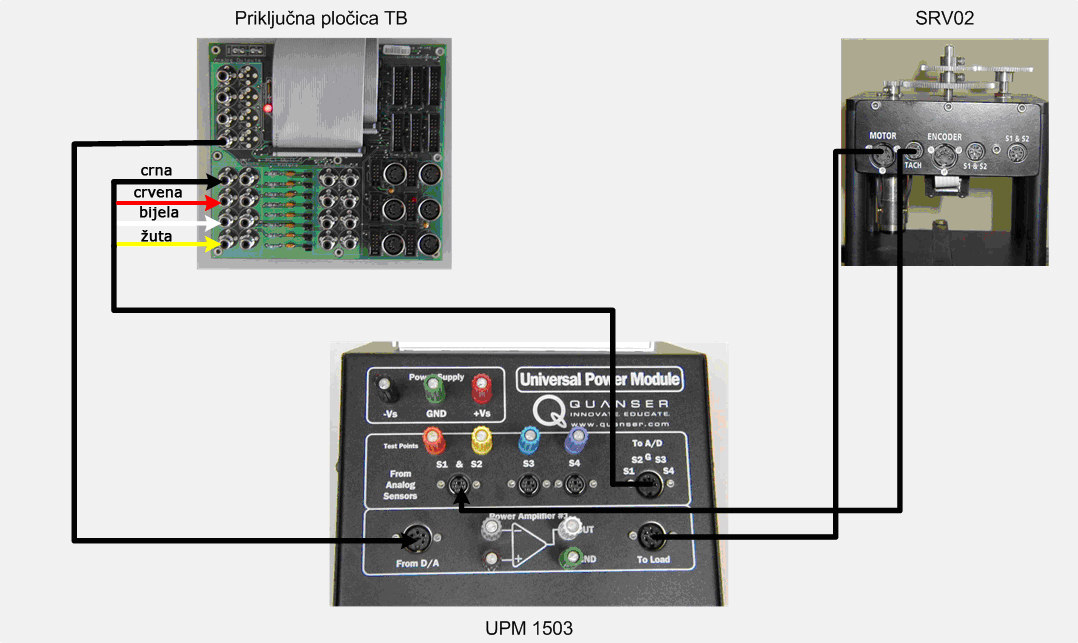
\includegraphics[width=0.8\textwidth] {konekcije.png}
    \caption{Shema spoja za implementaciju regulatora brzine vrtnje na realni elektromehanički sustav}
    \end{center}
\end{figure}

Na temelju sinteze regulatora provedene u vježbi 2., potrebno je izraditi algoritam regulacije brzine vrtnje, sl.2. Zbog potrebe usporedbe realnog i simuliranog odziva brzine vrtnje, u sklopu iste datoteke potrebno je izraditi i simulacijski model. Referentna vrijednost brzine zadaje se programski. Ona je zajednička za simulacijski dio i za dio algoritma koji upravlja realnim sustavom (SRV02), sl.2. Simulacijski model je identičan modelu u vježbi 2. 

Većina korištenih blokova u simulacijskom i realnom dijelu upravljačkog algoritma je identična. Jedina razlika je u tome što se u realnom dijelu upravljačkog algoritma umjesto SRV02 simulacijskog modela koristi realni proces, elektromehanički modul SRV02. Veza tog
realnog procesa s ostalim dijelovima sustava regulacije odvija se preko ulazno-izlaznog sučelja. U ovom slučaju to su jedan analogni izlaz i jedan analogni ulaz. Analogni izlaz prosljeđuje
upravljački signal prema energetskom pojačalu modula SRV02, dok se pomoću analognog ulaza prosljeđuje informacija s tahogeneratora prema upravljačkom algoritmu.

No prije nego što prijeđemo na generiranje upravljačkih algoritama i na finalnu shemu upravljanja realnog, odnosno simuliranog sustava pomoću referentne veličine i regulatora, potrebno je obratiti pozornost na određene izmjene u samim parametrima modela, pa tako i u parametrima regulatora za oba naša sustava.

\subsection{Nadopune modela i regulatora}

Kako su se parametri našeg sustava neznatno izmjenili, prije no što povežemo sustav s realnim modulom potrebno je obratiti pozornost kako izmjena parametara utječe na odziv našega sustava.

S obzirom da ne bi bilo poželjno koristiti regulatore iz druge laboratorijske vježbe na sustave koji imaju drugačije parametre, a s time i potrebe regulacije, moramo generirati nove regulatore, odnosno neznatno prilagoditi one koji su korišteni u drugoj laboratorijskoj vježbi.

\subsubsection{Promjene parametara}
Primjetimo da su parametri kod kojih je došlo do izmjena sljedeći:


\begin{itemize}
  \item Prijenosni omjer zupčanika sustava $K_g = 70$
  \item Ekvivalentni moment tromosti kod opterećenja $J_{eq} = 2\cdot10^{-3} \: [kg\cdot m^2]$ 
  \item Ekvivalentni koeficijent viskoznog trenja $B_{eq}  \:  [N\cdot m / \frac{rad}{s}]$
\end{itemize}

Primjetimo da je sasvim prirodno da se prijenosni omjer zupčanika promjenio pošto smo u drugoj vježbi simulirali brzinu vrtnje sustava promatranu na vanjskoj motornoj osovini, gdje je prijenosni omjer između unutarnje motorne i vanjske motorne osovine bio $14:1$, dok sada promatramo brzinu vrtnje sustava gledanu na osi pogonske osovine, gdje se prijenosni omjer povećava za veličinu zupčanika na pogonskoj osovini, odnosno $K_g = 14\cdot 5= 70$. Također, promjenom momenta tromosti $J_{eq}$ i koeficijenta viskoznog trenja $B_{eq}$, naš matematički model sustava poprilično se promijenio, te sada imamo novu prijenosnu funkciju našeg procesa:

\begin{equation}
G_p(s)=\frac{0.334}{0.0052\cdot s + 0.1834}
\end{equation}

\newpage

Uspredimo li to s prijenosnom funkcijom dobivenom modelom s parametrima iz druge laboratorijske vježbe:

\begin{equation}
G(s)=\frac{0.066796}{2.5441\cdot10^{-4}\cdot s + 0.01107966}
\end{equation}

lako vidimo da je razlika više nego uočljiva.
\newline
Ukoliko želimo vidjeti kako se naš sustav nosi s regulacijskim zahtjevima gdje za regulator koristimo onaj sintetiziran u drugoj laboratorijskoj vježbi. Odnosno:

\begin{equation}
G_r(s)=C(s)\cdot K_p \cdot \frac{1}{s} = \frac{41.5}{s} \cdot \frac{2.864\cdot s+100}{s+286.4}
\end{equation}

Dobivamo Bodeov dijagram prikazan na slici 2.2.

\begin{figure}[h]
	\begin{center}
	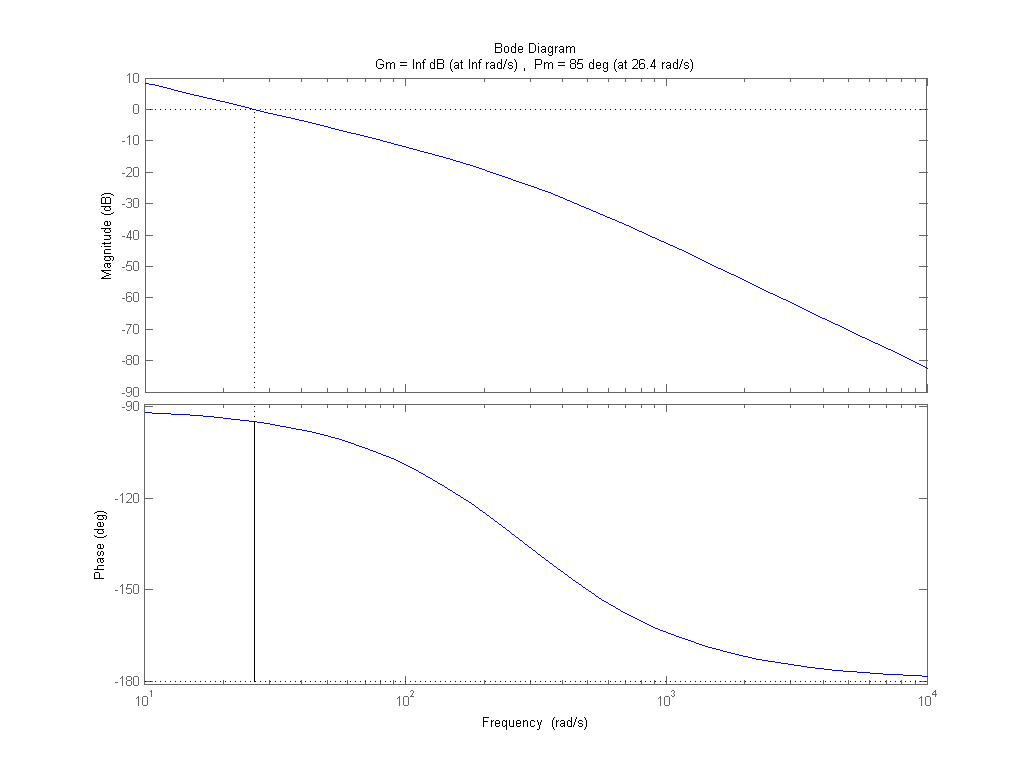
\includegraphics[width=0.8\textwidth]{bode_krivi_reg.png}
    \caption{Bodeov dijagram novog sustava uz neprilagođen regulator}
    \end{center}
\end{figure}

\subsubsection{Prilagođavanje regulatora}
Kako bi zadovoljili regulacijske zahtjeve zadane u \ref{sec:zahtjevi}, moramo prilagoditi naše regulatore da bolje odgovaraju novim prijenosnim funkcijama procesa.

Krećemo od statičkog pojačanja $K_p$, gdje iterativnim postupkom, kao i u drugoj laboratorijskoj vježbi, tražimo iznos za koji imamo presječnu frekvenciju na aproksimativno 100 rad/s. Zaključujemo da je zadovoljavajuće dobar za naše potrebe iznos pojačanja od $K_p \approx 165.5$.

Za navedeni iznos dobivamo Bodeov dijagram prema slici 2.3.

\newpage
\begin{figure}[h]
	\begin{center}
	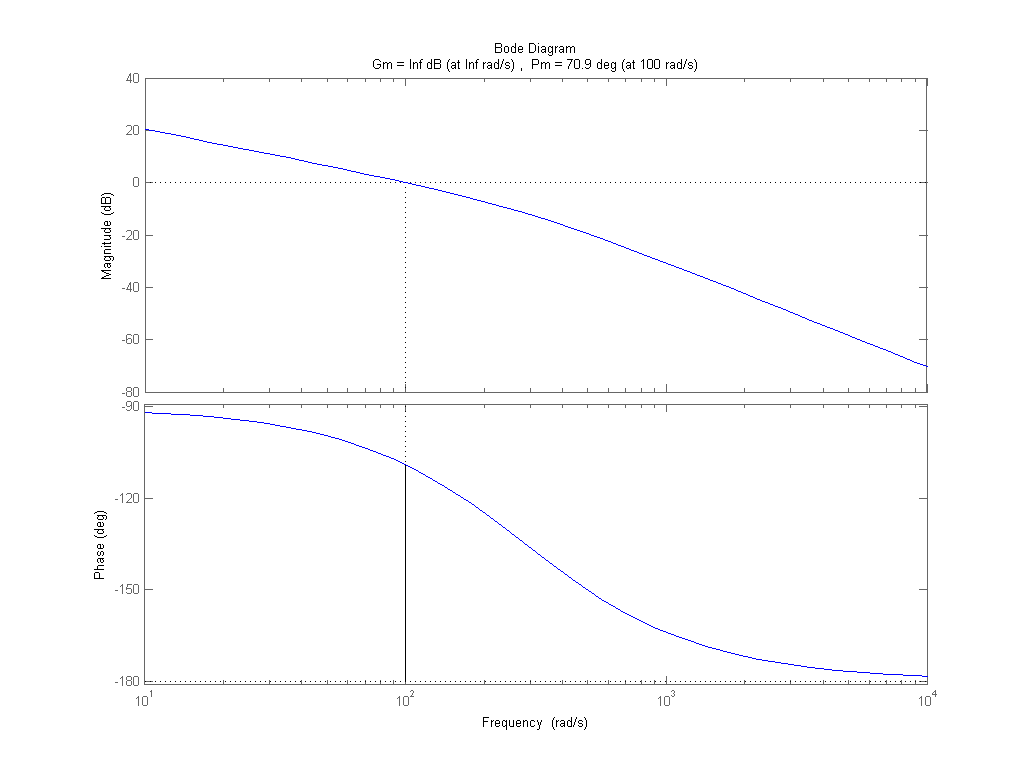
\includegraphics[width=0.8\textwidth]{bode_kp.png}
    \caption{Bodeov dijagram novog sustava uz prilagođeno pojačanje $K_p \approx 165.5$.}
    \end{center}
\end{figure}

Kako bi u potpunosti prilagodili naš model da bude što sličniji realnom rotacijskom modulu SRV02, moramo odrediti za koliko se izmjenio koeficijent viskoznog trenja $B_{eq}$. Kako je viskozno trenje inherentno mehanički parametar, njega određujemo usporedbom našeg modela i stvarnog modula, aproksimativnim postupkom.

Za početak stvorimo manju testnu funkciju za usporedbu odziva naša dva sustava, kao što je prikazano na slici 2.4.

\begin{figure}[h]
	\begin{center}
	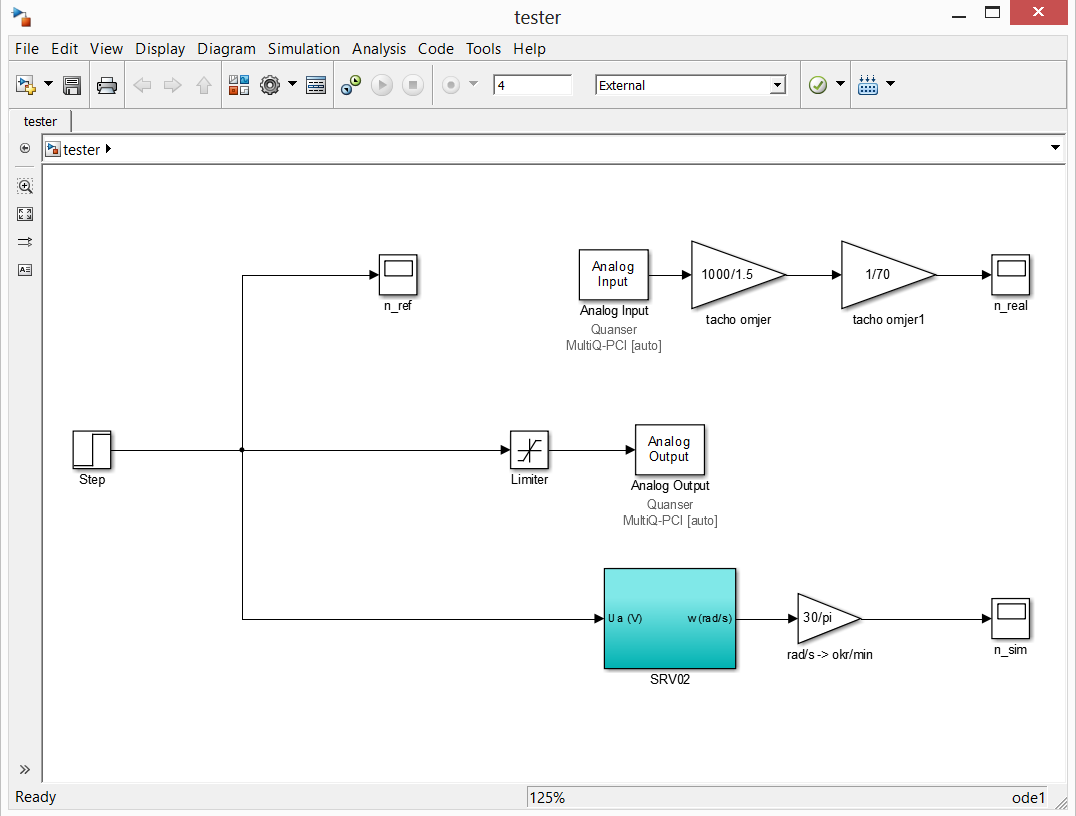
\includegraphics[width=0.7\textwidth, height = 3.3 in]{tester.png}
    \caption{Shema funkcije za iterativno određivanje koeficijenta viskoznog trenja $B_{eq}$}
    \end{center}
\end{figure}

\newpage

Pošto smo prije povezali MATLAB s našim realnim sustavom, daljnje određivanje viskoznog trenja $B_{eq}$ svodi se na iteriranje simulacije, odnosno mjerenja i mjenjanje parametra $B_{eq}$ dok ne postignemo da su nam odzivi stvarnog i simuliranog sustava što sličniji.

Iteriranjem dolazimo do odziva prikazanog na sljedećoj slici.

\begin{figure}[h]
	\begin{center}
	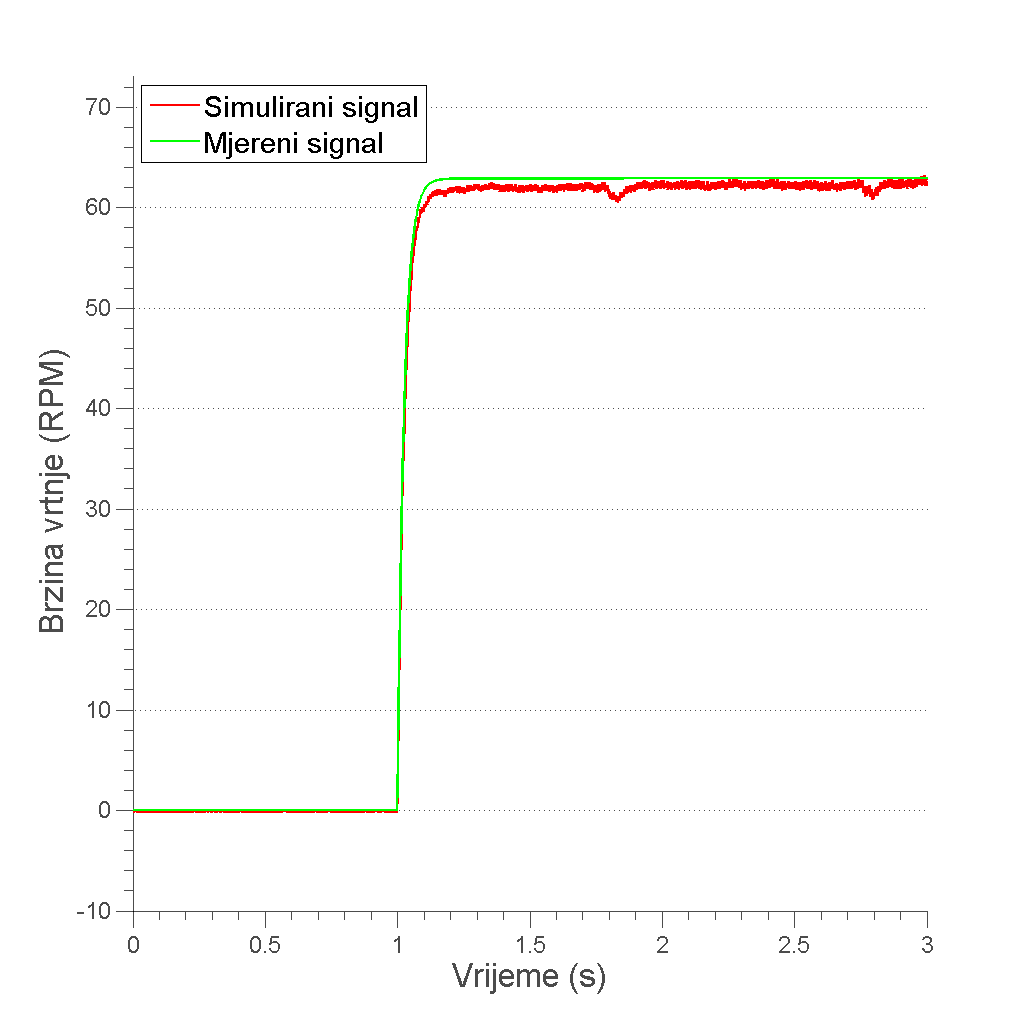
\includegraphics[width=0.7\textwidth]{tester_odziv.png}
    \caption{Usporedba simuliranog i mjerenog signala pri $B_{eq} = 0.009$}
    \end{center}
\end{figure}

Isti dobivamo za viskozno trenje iznosa $B_{eq}B = 0.009$, odnosno šest puta većeg iznosa nego što smo imali u drugoj laboratorijskoj vježbi.

Time smo uspješno odredili nove parametre našeg modela sustava, te prilagodili regulator na način da naš novi sustav ispunjava zahtjeve zadane u \ref{sec:zahtjevi}.

Možemo nastaviti s izvođenjem mjerenja.


\subsubsection{Upravljački algoritam}

Kako bi mogli usporediti odzive mjerenog i simuliranog sustava te koliko dobro oni prate referentnu veličinu brzine vrtnje, kreiramo Simulink model, odnosno korisnički algoritam, prema shemi na slici 2.6.

\newpage

\begin{figure}[ht]
	\begin{center}
	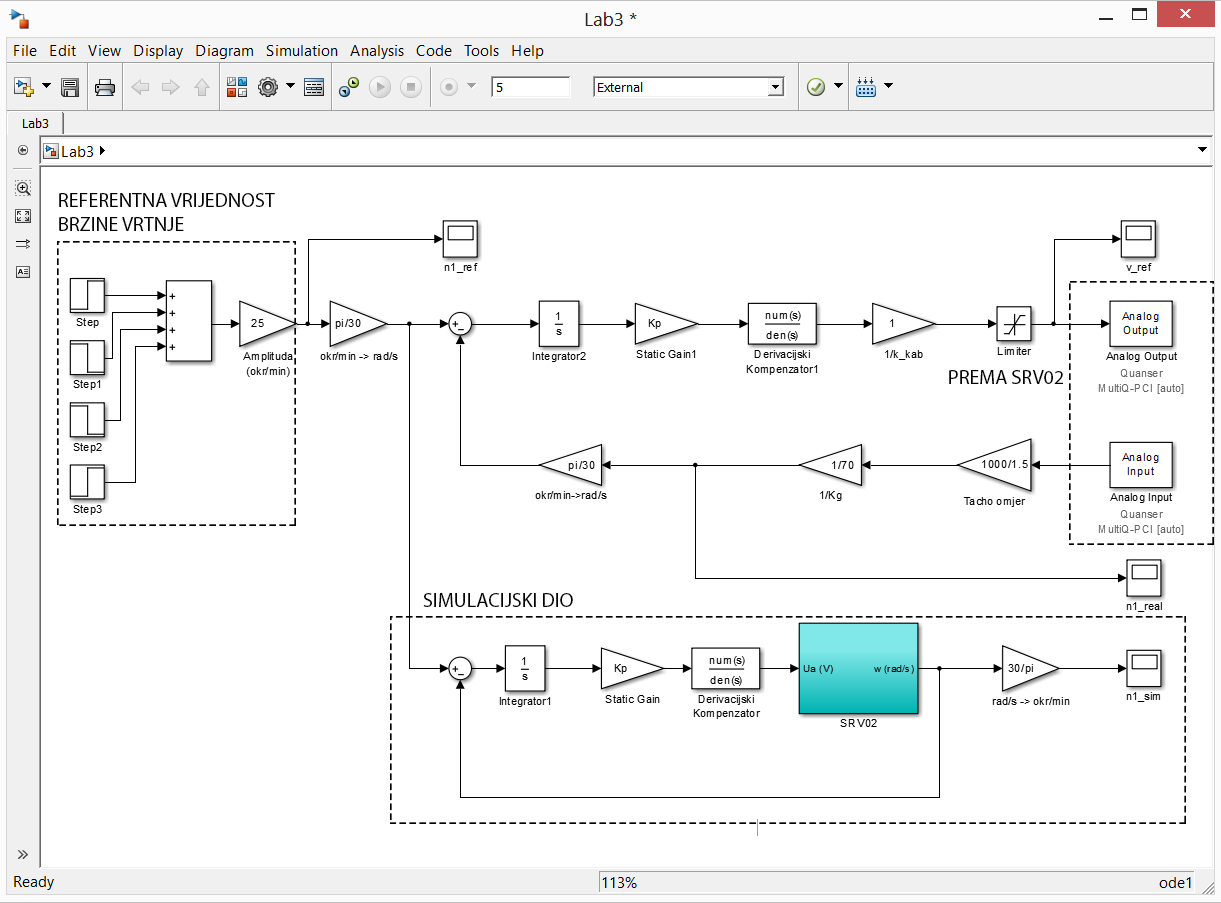
\includegraphics[width=0.8\textwidth]{simulator_oznake.png}
    \caption{Prikaz korisničkog algoritma (sa simulacijskim modelom za usporedbu) za sustav regulacije brzine vrtnje}
    \end{center}
\end{figure}

Gdje je ulazni parametar brzine vrtnje definiran prema funkciji prikazanoj na slici 2.7.


\begin{figure}[!h]
	\begin{center}
	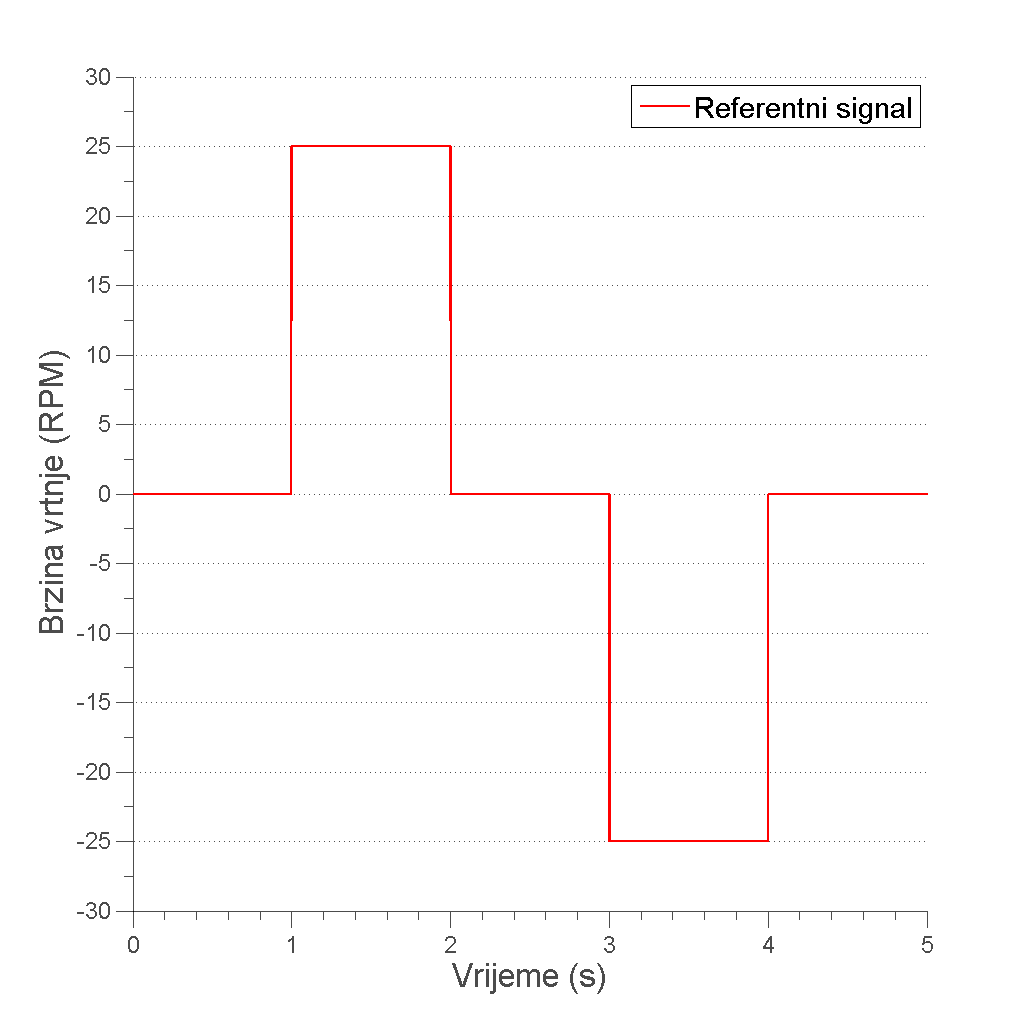
\includegraphics[width=0.8\textwidth, height = 4in]{ulazna_f.png}
    \caption{Ulazna funkcija brzine vrtnje s amplitudom 25}
    \end{center}
\end{figure}

U nastavku, testiramo naš sustav te komentiramo odzive.

\newpage


\subsection{Rezultati mjerenja i simulacije}


Izvođenjem našeg algoritma upravljanja na realan model, odnosno simulacijom za zadani regulator na matematičkom modelu dobivamo sljedeće odzive.

\begin{figure}[h]
	\begin{center}
	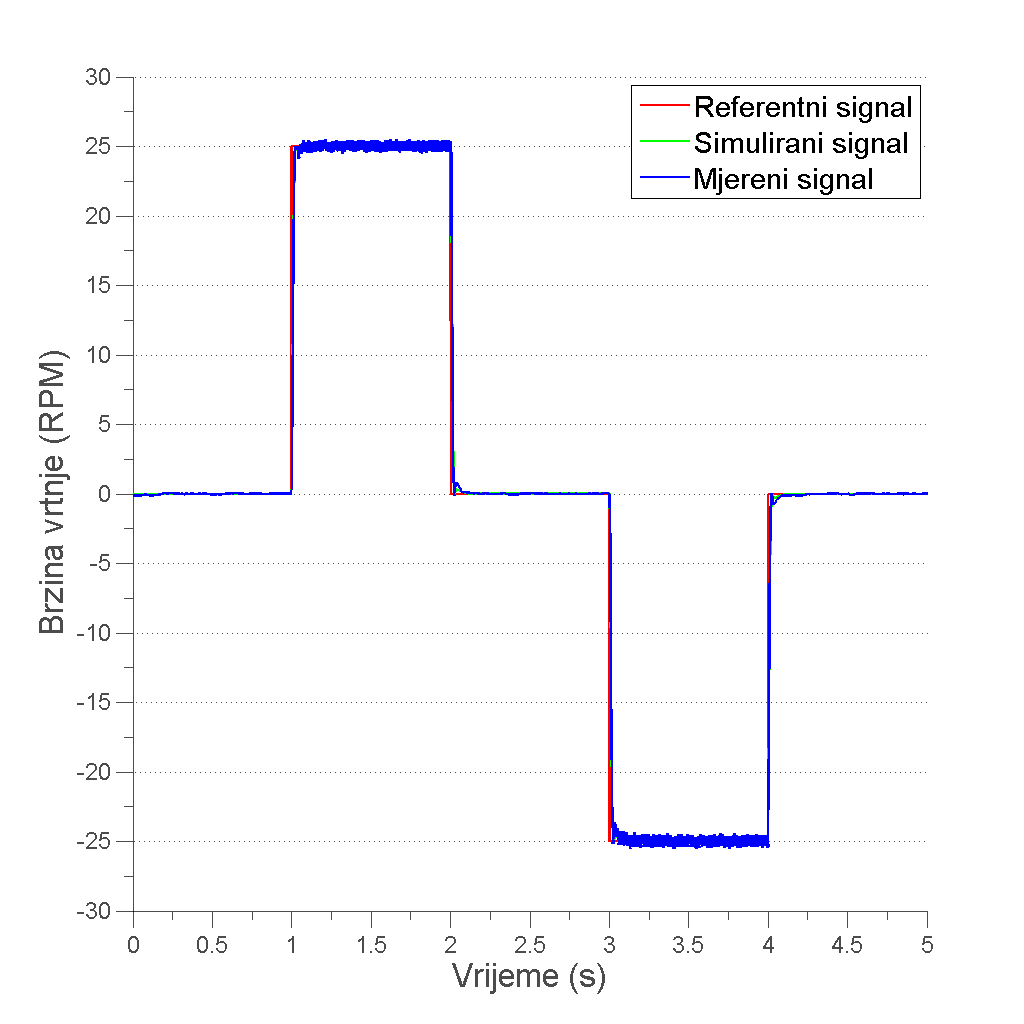
\includegraphics[width=0.8\textwidth]{Odziv_6x_2.png}
    \caption{Odziv simuliranog i mjerenog sustava na referentni signal brzine vrtnje}
    \end{center}
\end{figure}


Već ovdje vidimo da naš mjereni i simulirani sustav relativno vjerno prate referentnu veličinu. Dakako, nas ne zanima generalno praćenje, nego koliko dobro oba sustava ispunjavaju regulacijske zahtjeve.

Pogledajmo uvećan prikaz ovog odziva na slikama 2.9. i 2.10.

\newpage

\begin{figure}[!ht]
	\begin{center}
	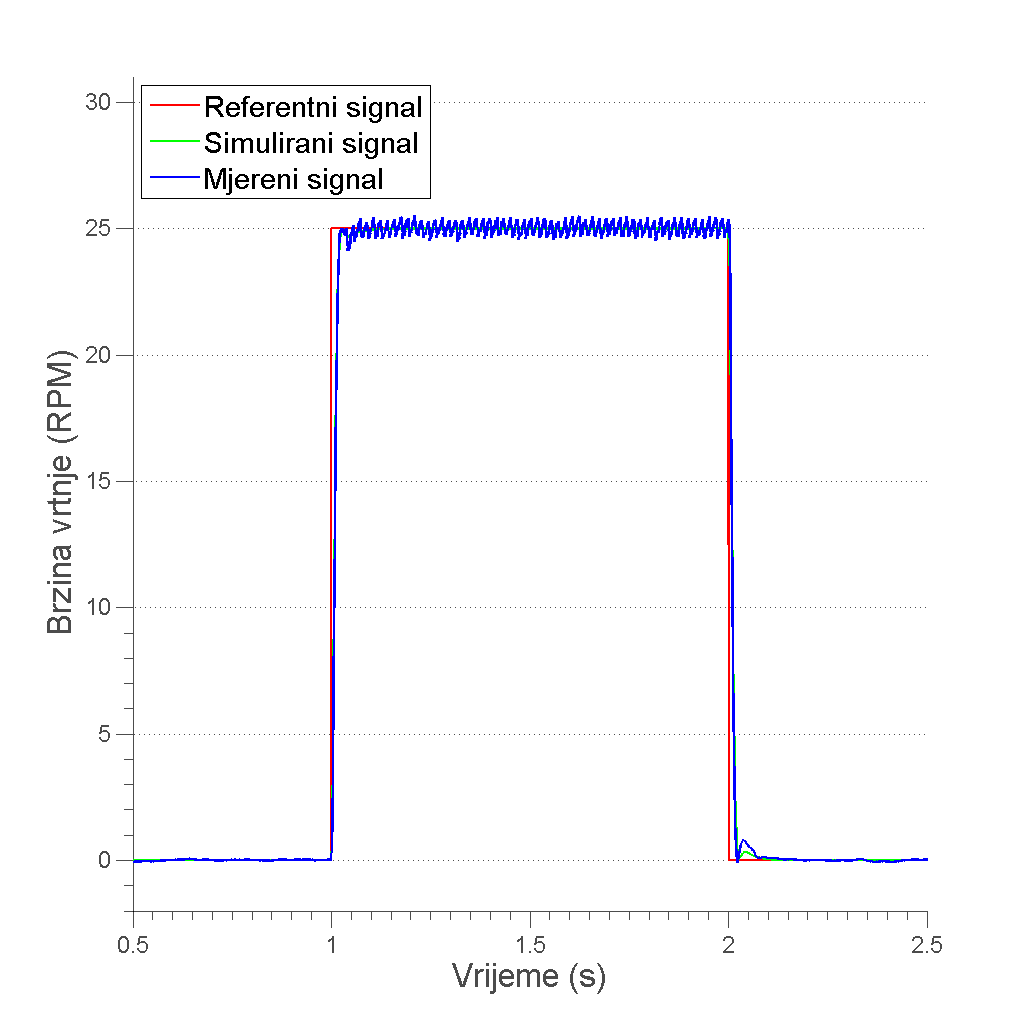
\includegraphics[width=0.8\textwidth, height=4in]{Odziv_6x_halfclose.png}
    \caption{Odziv simuliranog i mjerenog sustava na referentni signal brzine vrtnje, uvećan prikaz}
    \end{center}
\end{figure}

\begin{figure}[!hb]
	\begin{center}
	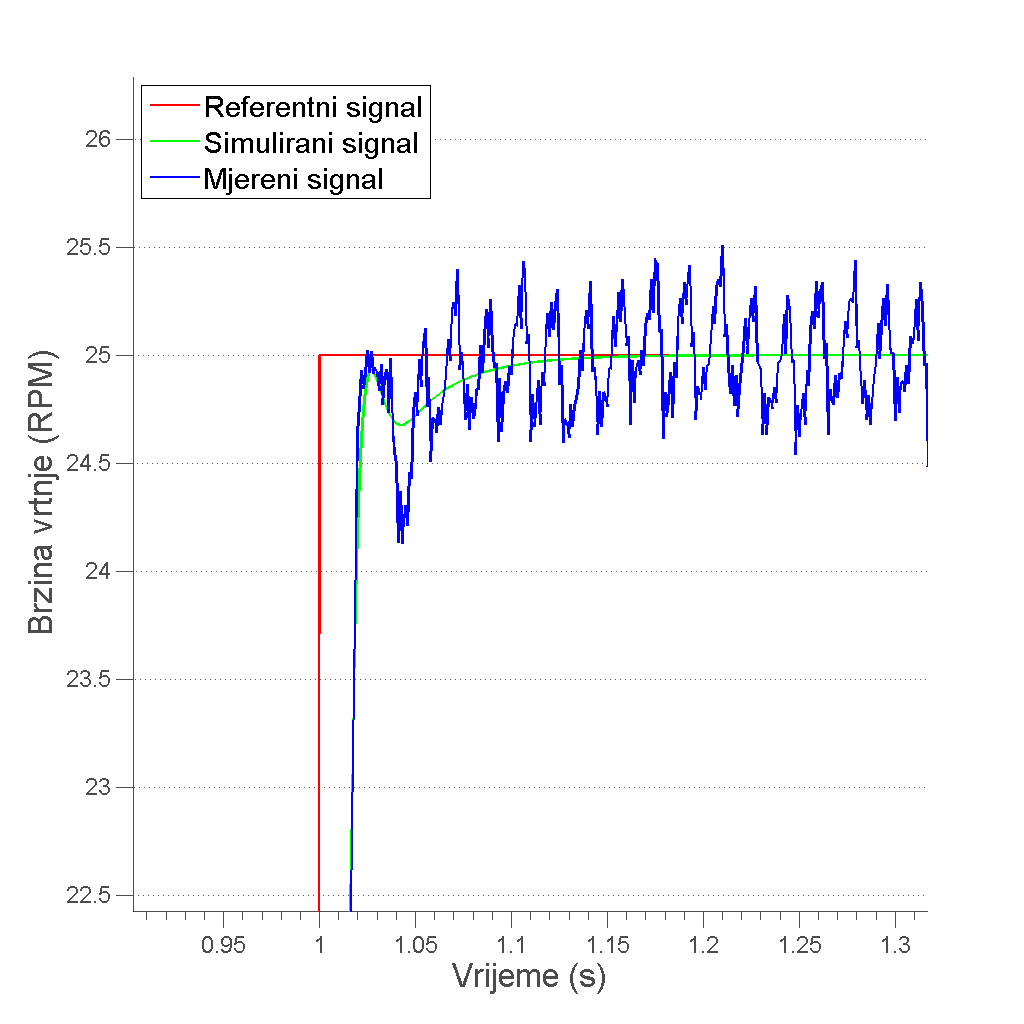
\includegraphics[width=0.8\textwidth, height=4in]{Odziv_6x_close_2.png}
    \caption{Odziv simuliranog i mjerenog sustava na referentni signal brzine vrtnje, prijelazna pojava}
    \end{center}
\end{figure}

\newpage

Vidimo da sustav nema nadvišenja, te iako signal iz tahogeneratora oscilira oko referentne veličine, on dobro prati referentni signal.
Oscilacije kod tahogeneratora posljedica su mjernih pogrešaka koje nastaju usred fizikalnih oštećenja ležajeva u kučištu motora, kao i malih fluktuacija u signalu tahogeneratora. S obzirom da tahogenerator daje signal u milivoltima, te isti moramo množiti s koeficijentom 1000/1.5 da bi dobili okretaje u minuti, ovakve oscilacije ne iznenađuju.


\subsection{Opažanja i zaključci}

Tokom izvođenja pokusa uvidjeli smo da korištenjem prilagođenog regulatora oba naša sustava zadovoljavajuće dobro prate referentnu veličinu, te poštuju sve regulacijske zahtjeve zadane u \ref{sec:zahtjevi}

Naravno, uvijek možemo dalje prilagođavati naš regulator prema nekim kriterijima koje si zadamo, iako svako poboljšanje u određenom smjeru nužno za sobom nosi više ili manje poželjne posljedice, poput (ne)stabilnosti u stacionarnom stanju, produženog vremena istitravanja, mogućeg nadvišenja i slično.

Regulacijski zahtjev, da se presječna frekvencija nalazi na 100rad/s, jednoznačno određuje granicu frekvencije ulazne funkcije sustava. Razlog tomu je što smo određivanjem presječne frekvencije osigurali da se prvi maksimum postiže nakon izvjesnog vremena. Ta relacija je empirijski određena, te u našem primjeru iznosi aproksimativno 0.03 sekunde.


\begin{figure}[!h]
	\begin{center}
	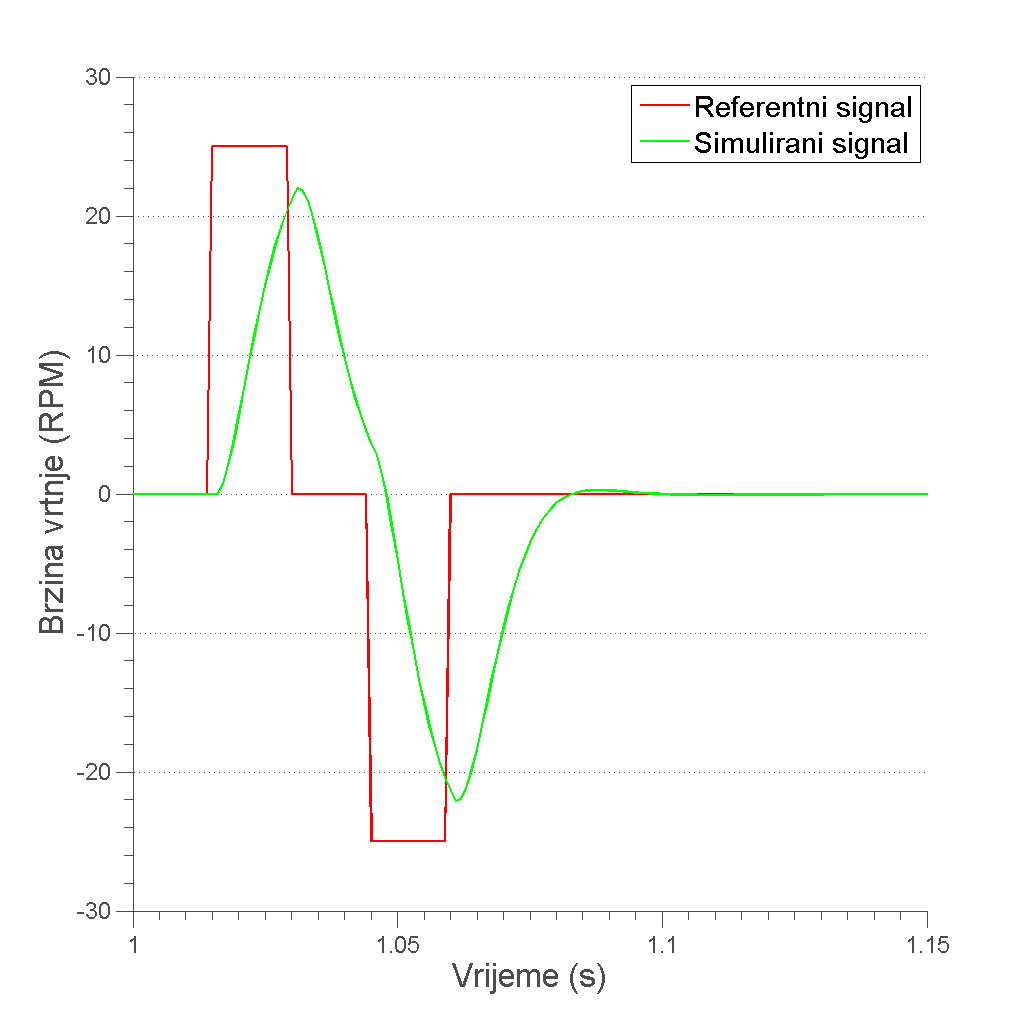
\includegraphics[width=0.8\textwidth]{ogranicenje_2.png}
    \caption{Odziv simuliranog sustava pri frekvenciji ulazne funkcije iznosa $f=166 Hz$}
    \end{center}
\end{figure}

\newpage 

Ukoliko je frekvencija ulazne funkcije viša od tog iznosa, odnosno prijelazi se događaju brže od 0.03 sekunde, možemo očekivati da odziv sustava nikada neće postići vrijednost maksimuma referentnog signala, te će u odzivu konstantno kaskati za istim.
\newline
Tu pojavu možemo vidjeti na slici 2.11.

Nadalje, ukoliko povećamo amplitudu funkcije ulaznog signala, karakteristike sustava bit će narušene s obzirom da regulator nije projektiran za te namjene. Očituje se izraženim nadvišenjem sustava pri spuštanju na brzinu vrtnje od 0 rad/s.
Osim  regulatora, ni naš simulacijski model nije prilagođen promjeni amplitude funkcije ulaznog signala. S obzirom da je iznos viskoznog trenja $B_{eq}$, dobiven iterativnim putem, te on predstavlja viskozno trenje mehaničkog sustava pri određenoj brzini vrtnje, za očekivati je da će model biti neprecizan ukoliko se amplituda ulazne funkcije, odnosno brzina vrtnje sustava, zamjetno promjeni. Ukoliko je viskozno trenje neadekvatno postavljeno, to se očituje statičkom pogreškom između mjerenog i simuliranog odziva sustava.

Ukoliko imamo ova ograničenja na pameti te prilagođavamo parametre simulatora po potrebi, zaključujemo da tada naš simulator vjerno opisuje rad rotacijskog elektromehaničkog modula SRV02 na ulaznu pobudu.



\end{document}




%Na vlastitu odgovornost...
